\section*{S7.2(C)}
\begin{figure}[H]
\centering
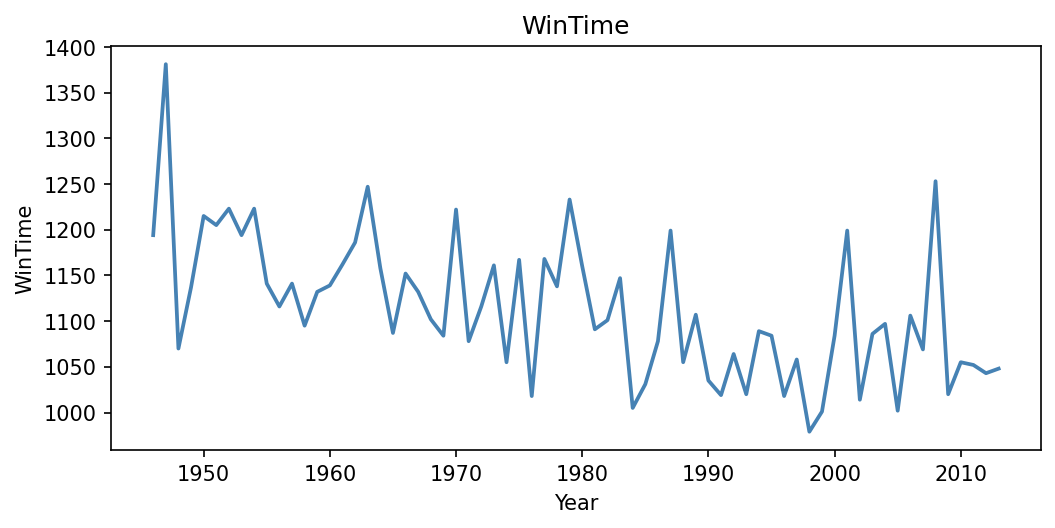
\includegraphics[width=0.95\linewidth]{S7.2C_wintime.png}
\caption{Time-series plot of WinTime}
\end{figure}
\begin{figure}[H]
\centering
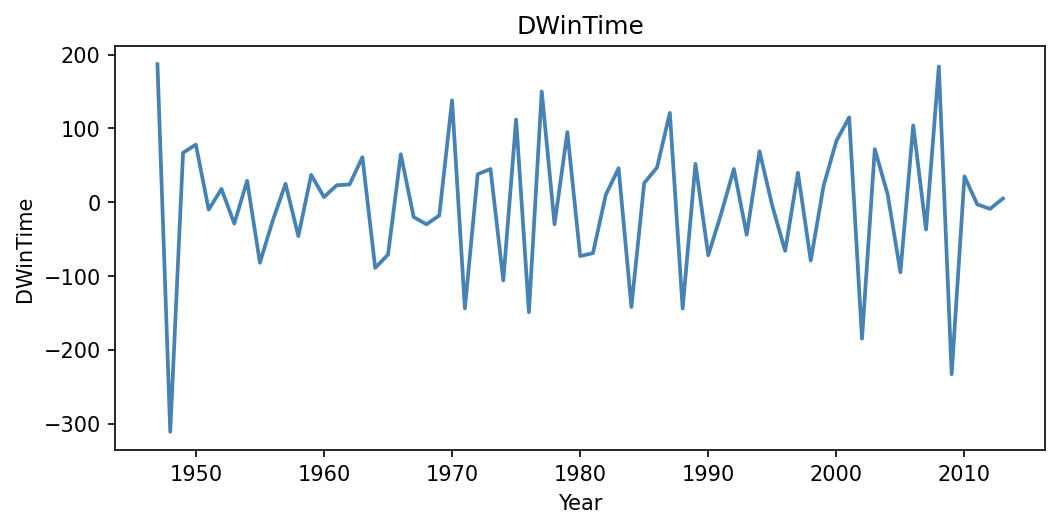
\includegraphics[width=0.95\linewidth]{S7.2C_dwintime.png}
\caption{Time-series plot of DWinTime}
\end{figure}
\begin{figure}[H]
\centering
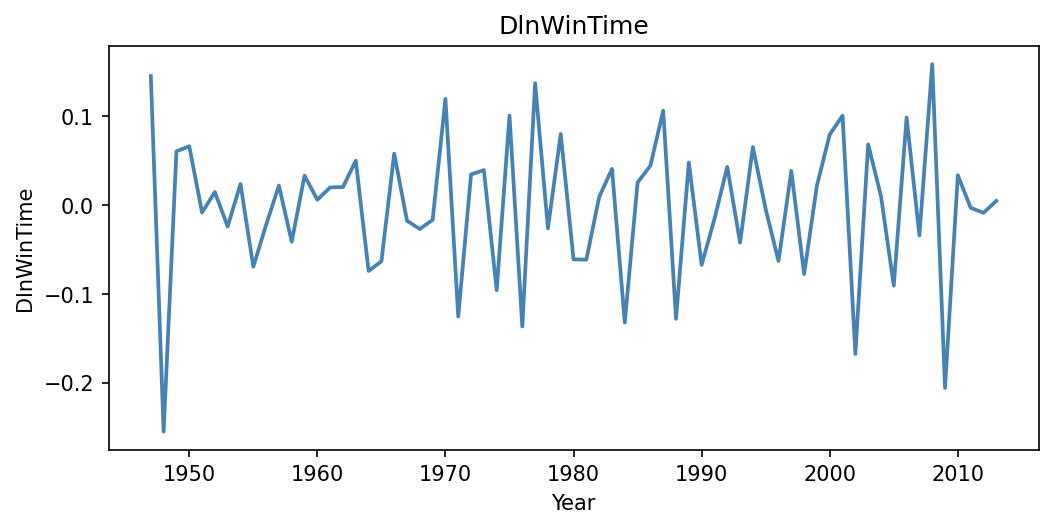
\includegraphics[width=0.95\linewidth]{S7.2C_dlnwintime.png}
\caption{Time-series plot of DlnWinTime}
\end{figure}
WinTime shows moderate long-run variation with no obvious deterministic trend; year-to-year changes appear noisy. 
The first difference DWinTime fluctuates around zero with occasional spikes, suggesting short-run shocks. 
The log-difference DlnWinTime similarly centers near zero and compresses large swings, indicating proportionate changes are small and mean-reverting.
\begin{figure}[H]
\centering
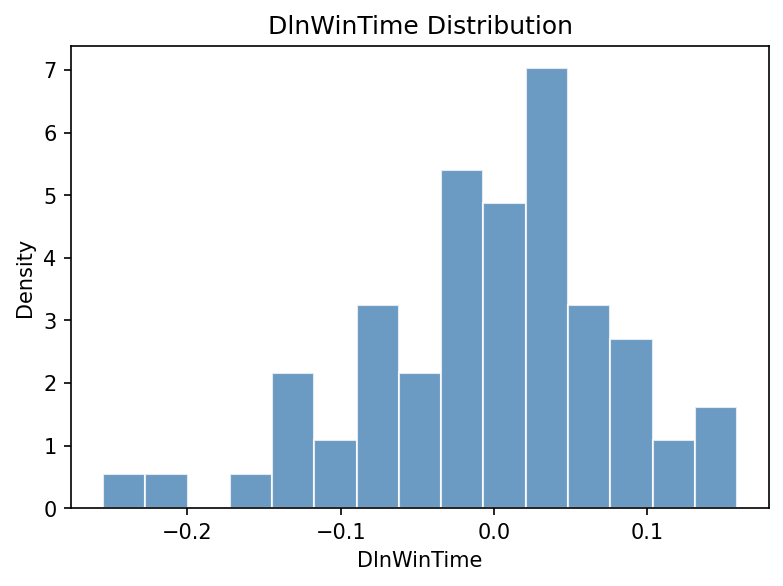
\includegraphics[width=0.75\linewidth]{S7.2C_dlnwintime_dist.png}
\caption{Distribution of DlnWinTime (histogram, density)}
\end{figure}
